\documentclass{article}
\usepackage[utf8]{inputenc}
\usepackage{graphicx}
\graphicspath{{images/}{../images/}}

\title{Secure Programming Summary}
\author{j.s.burley }
\date{November 2018}

\begin{document}

\maketitle

\tableofcontents
\newpage
\section{Introduction}
\subsection{What is security?}
The state of being secure
\\CIA: \textbf{only} authorised actors can:
\begin{itemize}
    \item Learn secrets (\textbf{Confidentiality})
    \begin{itemize}
        \item \textbf{Data Confidentiality}: make sure that private information is not available to unauthorised actors
        \item \textbf{Privacy}: Individuals have control over what information is collected and stored, and how that information is shared
    \end{itemize}
    \item Modify messages/data (\textbf{Integrity})
    \begin{itemize}
        \item \textbf{Data Integrity}: Assures that information is modified only in a way that is known
        \item \textbf{System Integrity}: Ensures that a system performs as designed, without unauthorised modification
    \end{itemize}
    \item Access messages/data (\textbf{Availability})
    \begin{itemize}
        \item \textbf{Availability}: ensures that service is provided to an acceptable level, without denying access to authorised users
    \end{itemize}
\end{itemize}
Security is best \textbf{by design} - not as afterthought
\subsection{Identifying requirements for a secure protocol}
\begin{itemize}
    \item Always work towards CIA protocols described above
    \item We can do this by using the following three techniques
    \begin{itemize}
        \item Cryptographic algorithms to hide, sign and provide guarantees about messages
        \item Use cryptography in protocols, systems in order to secure them
        \item Program with security in mind in order to avoid exploits that may manipulate software
    \end{itemize}
    \item An additional requirement is \textbf{Non-repudiation}: One party of a transaction cannot deny having received a transaction, nor can the other party deny having sent the transaction.
\end{itemize}
Access Control
\begin{itemize}
    \item \textbf{Identification}: A user states their identity (i.e. a username)
    \item \textbf{Authentication}: The system verifies this identity (i.e. through a shared secret like a password)
    \item \textbf{Authorisation}: This user is authorised to perform a particular task, or access a particular file
\end{itemize}
\section{Cryptology}
Cryptography: The mathematics of secret communication
\\Cryptology: Includes study of breaking cryptographic protocols (known as cryptanalysis)
\\The challenge of cryptology is to map mathematics of cryptosystems onto computers with the help of engineers
\subsection{Basic Concepts}
\textbf{Kerckhoff's Principle}: A cryptosystem should be secure \textit{even if} everything about the system, \textit{except the key} is public knowledge.
\\There is no "Security by obscurity": all crypto algorithms are assumed to be known. Security is based on:
\begin{itemize}
    \item Secrecy of the key
    \item Hard to infer the plaintext from the cipher text
\end{itemize}
\textbf{Cryptanalysis} is inferring the plaintext from ciphertext \textit{without} knowing the key.
\subsection{Examples of ciphers}
\subsubsection{Caesar Cipher}
\begin{itemize}
    \item Monoalphabetic substitution cipher
    \item Key is a constant shift (i.e. 5 letters)
    \item We encrypt by shifting each message letter by $key$ letters (AAA -> FFF)
    \item ROT13 is least secure variant of this: shift by 13 letters. ROT13 is its own inverse
\end{itemize}
It is easy to break monoalphabetic substitution ciphers using techniques like frequency analysis of the most common letters in a given language. We can then perform frequency analysis on the message to determine if there is a letter that matches the frequency of one in the message language.
\subsubsection{Vigenére Cipher}
\begin{itemize}
    \item Polyalphabetic substitution cipher
    \item We use a table called a \textit{tabula recta}
    \item Has multiple keys
    \item Repeat the keys for the length of the message, use the table to determine which letter to substitute
\end{itemize}
We can break polyalphabetic ciphers by breaking the message into components and grouping ciphertexts into parts corresponding to each key character. We can then use frequency analysis on each of these message components.
\subsubsection{One Time Pad}
\begin{itemize}
    \item Takes concept of Vigenére to the extreme
    \item Key size = plaintext size (or larger) in order to avoid repeated patterns
    \item Only known algorithm with perfect secrecy
    \item Key distribution is a problem (have to keep key secret, prevent interception)
    \item If random key is never re-used as a whole or in part, and kept completely secret, impossible to use cryptanalysis to break it.
\end{itemize}
\subsubsection{Block ciphers}
With the above methods, we treat messages as a one-dimensional stream, and we either substitute or shift letters to encrypt. With \textbf{Block Ciphers}, we include transpositions.
\subsubsection{Playfair Cipher}
\begin{itemize}
    \item simple block cipher from 1854 (unsafe nowadays)
    \item Key is a 5x5 matrix with the keyphrase (we replace I with J so the alphabet fits)
    \item encrypt messages in digrams (two letter pairs)
    \item pad the message if a digram is incomplete, or if a digram consists of two of the same letter (X is a common padding letter)
\end{itemize}
Rules of playfair:
\begin{enumerate}
    \item If two letters are in the same row or column, replace by shifting the letter to the right (row) or down (column). Use wrap around if there is no letter directly to the right of a chosen letter.
    \item Otherwise, picture a rectangle formed by the two letters. Replace the letters with those at the two "unoccupied" corners of that rectangle. The order for this is important: first letter of ciphertext pair must come from the same \textbf{row} as the first letter of the plaintext pair.
\end{enumerate}


\subsection{Symmetric Encryption}
\subsubsection{Symmetric Ciphers}
\begin{itemize}
    \item relatively fast
    \item One key to encrypt and decrypt
    \item block vs stream variants
    \item has a major weakness: \textbf{key distribution}
\end{itemize}
\subsubsection{Modern Symmetric Ciphers}
Typically injective (one-to-one) to allow for decryption
\\Vulnerable to statistical attacks, as small blocks can only take limited transformations
\\large blocks are impractical
\\Key size can grow quite large: 4 bits x 16 rows
\\in general, n x $2^n$, so a 64-bit block would require a key of 64 x $2^64 = 10^21$ bits (125 Exabytes, 125,000 petabytes)
\begin{itemize}
    \item DES, 3DES, AES (AES most dominant, DES broken)
    \item based on substitution and transposition
    \item too complex to do by hand
    \item block ciphers (DES, 3DES, AES,...)
    \item also stream ciphers, the most well known being RC4
\end{itemize}
\subsubsection{Block vs Stream}
\begin{itemize}
    \item Block ciphers: block of plaintext treated as a whole and produces a ciphertext block (typically of equal length). Typical length is 64 or 128 bits. Achieved using substitution and transposition. Diffusion \& confusion
    \item Stream ciphers: encrypts a digital data stream 1 bit/byte at a time, no regard for padding or length
\end{itemize}
\subsubsection{Diffusion vs Confusion}
\begin{itemize}
    \item diffusion: each plaintext digit affects the value of many ciphertext digits with a cascade effect
    \item confusion: statistics of ciphertext and value of the encryption key are as complex as possible
\end{itemize}
\subsubsection{Transposition cipher}
Permutation over a block of plaintext.
\begin{verbatim}
Key:        4312567
Plaintext:  attackp
ostpone
duntilt
woamxyz
\end{verbatim}
If you read the characters column-wise in the order provided by the key, you get the following message:
\begin{verbatim}
ttna aptm tsuo aodw coix knly petz
\end{verbatim}
Putting this together, we get the nonsense string:
\begin{verbatim}
ttnaaptmtsuoaodwcoixknlypetz
\end{verbatim}
\subsubsection{Feistel Cipher}
\begin{itemize}
    \item Goal: approximate ideal cipher and reduce statistical properties linking plaintext, ciphertext and keys
    \item Combining substitutions and permutations: each plaintext element or group of elements is uniquely replaced by a corresponding ciphertext element or group of elements, and a sequence of plaintext elements is replaced by a permutation of that sequence. No elements are added or deleted or replaced in the sequence, but the order of the elements in the sequence is changed.
\end{itemize}
\textbf{Substitution:} right part of plaintext block transformed by F(Ki) and XORed with left part
\\\textbf{Permutation:} right part swapped with left part
\\Relationship between the $i^{th}$ round and the output of the previous round given by:
$$L_i = R_{i-1}$$
$$R_i = L_{i-1}\bigoplus f(K_i, R_{i-1})$$
where $f$ is called the Feistel function.
\textbf{Properties}
\begin{itemize}
    \item \textbf{Block size:} larger blocks mean greater security but lower encrypt/decrypt speed. Block size of 64 is a reasonable tradeoff, AES uses 128
    \item \textbf{Key size:} larger key = greater security but reduced encrypt/decrypt speed. 64-bit key size is considered inadequate, 128bits common
    \item \textbf{Number of rounds:} essence of feistel cipher is that a single round is not secure enough, multiple rounds increase security. 16 rounds is typical
    \item \textbf{Round key generation algorithm:} greater complexity in this algorithm -> greater difficulty of cryptanalysis
    \item \textbf{Round function F:} greater complexity in this algorithm -> greater difficulty of cryptanalysis
\end{itemize}
\textbf{Extra (desired) properties}
\begin{itemize}
    \item \textbf{Fast software encryption/decryption:} encryption is often embedded in applications or utility functions to avoid a hardware implementation
    \item \textbf{ease of analysis:} If algorithm is easier to analyze, it is easier to find (cryptanalytic) vulnerabilities and strengthen algorithm. (i.e. DES is not easily analyzed)
\end{itemize}
\textbf{Block modes}
\\\textbf{Electronic codebook (ECB)}
\begin{itemize}
    \item each block is encoded independently using the same key
    \item used for: secure transmission of single blocks (i.e. an encryption key)
    \item \textbf{identical blocks can leak information or lead to attacks!}
\end{itemize}
\textbf{Cipher Block Chaining (CBC)}
\begin{itemize}
    \item input to the encryption algorithm is the XOR of the next 64 bits of plaintext and the preceding 64 bits of ciphertext
    \item used for: general purpose block-oriented transmission
    \item Requires initialization vector (IV) to XOR with the first plaintext block
\end{itemize}
There are others: PCBC, CFB, OFB, CTR.
\\\textbf{Choosing the wrong block mode is a major factor in implementation weaknesses}
\subsubsection{DES}
\begin{itemize}
    \item 64 bit block size
    \item key length is 56 bits, with 8 bits for parity (64 bits total)
    \item 16 round feistel structure
\end{itemize}
\subsubsection{AES}
\begin{itemize}
    \item subset of \textit{Rijndael}, developed in 1998 by two belgian cryptographers John Daemen and Vincent Rijmen
    \item most widely used symmetric cipher today
    \item 128 bit block size
    \item 128, 192 or 256 bit key size
\end{itemize}
\section{Public Key Crypto Systems}
\begin{itemize}
    \item public-key/two-key/asymmetric crypto involves the use of two keys
    \item \textbf{public key:} may be known to anyone, and can be used to encrypt messages and verify signatures
    \item \textbf{private key:} known only to the recipient, used to decrypt messages and create signatures
    \item \textbf{asymmetric because:} encryptors and verifiers cannot decrypt or create signatures
    \item {PKCS: Public Key Crypto Standards}
\end{itemize}
\subsection{Why do we use it?}
Addresses two key issues:
\begin{itemize}
    \item \textbf{Key distribution:} how to have secure communications in general without having to trust the channel when transmitting symmetric key
    \item \textbf{digital signatures:} how do we verify a message comes (intact) from the claimed sender?
    \item Publicly invented by Whitfield Diffie and Martin Hellman in 1976, although existence of concept was known prior
\end{itemize}
It also has some useful features
\begin{itemize}
    \item can be used to transmit message securely
    $$C = E(M,P_{pu})$$
    $$M = D(M,P_{pr})$$
    Where C is ciphertext, M is message, and E and D are decrypt with P as the public and private key
    \item can also be used for authentication using a combination of pubkey/privkey encryption/decryption
    $$C' = E(M,P^{A}_{pu})$$
    $$C = E(M||C',P^{B}_{pu})$$
\end{itemize}
\subsection{Characteristics}
pubkey algorithms rely on two keys where:
\begin{itemize}
    \item its computationally infeasible to find decryption key knowing only algorithm and encryption key
    \item computationally easy to en/de-crypt messages when relevant key is known
    \item (for some algorithms) either key can be used to encrypt, with private required to decrypt
\end{itemize}
\subsection{RSA}
by Rivest, Shamir and Adleman of MIT in 1977
\\best known, most widely used pubkey scheme
\\based on exponentiation in a finite (Galois) field over integers modulo a prime (exponentation takes $O((log n)^3)$ operations, computationally easy)
\\uses large (1024 bits) integers
\\security through cost of factoring large numbers (factorization takes $O(e^{log n log n log n}$ operations, computationally hard)
\subsubsection{Setting up an RSA key}
Each user must generate a public/private key pair by:
\begin{itemize}
    \item Selecting two large primes at random - $p, q$
    \item compute their modulus $n=p\times q$, where $\phi(n)=(p-1)(q-1)$ \footnote{$\phi(n)$ being Euler's totient function: the number of integers $1 \leq k \leq n$ that are relatively prime to $n$}
    \item select at random the encryption key $e$ where $1 < \phi(n)$, $gcd(e,\phi(n)) = 1$
    \item solve the following equation to find decryption key $d$: $e \times d = 1 mod \phi(n)$ and $0<d<\phi(n)$
\end{itemize}
Users publish their encryption key: $PU ={e,n}$
\\Users keep private decryption key secret: $PR={d,n}$
\subsubsection{RSA usage}
To \textbf{encrypt} a message M, the sender:
\begin{itemize}
    \item Obtains the \textbf{public key} of recipient $PU$
    \item Computes: $C=M^e mod n$, where $0\leq M < n$
\end{itemize}
To decrypt the ciphertext C, the receiver:
\begin{itemize}
    \item uses their \textbf{private key} $PR={d,n}$
    \item computes: $M = C^d mod n$
\end{itemize}
\textit{note: message M must be smaller than modulus n (split message into blocks if necessary)}
\subsubsection{Why does RSA work like this?}
\textbf{Euler's totient function}
Expressed as $\phi(n)$ or $\varphi(n)$
\\Defined as the number of positive integers less than n and relatively prime to n
\\$\varphi(1) = 1$
\\Given that $n=pq$, and $p$ and $q$ are prime numbers:
$$\varphi(n)=\varphi(pq)=\varphi(p)\varphi(q)=(p-1)(q-1)$$
\textbf{Euler's theorem}
$\alpha, n$ relative prime: the only positive integer that evenly divides both is 1
$$\alpha^{\phi(n)}\equiv 1(mod n)$$
\textbf{So why does RSA work?}
Because of Euler's theorem:
$$a^{\phi(n)}mod n = 1$$ where $gcd(a,n)=1$
\\in RSA we have:
$$n=p\times q$$
$$\phi(n)=(p-1)(q-1)$$
we carefully choose $e$ and $d$ to be inverses $mod\phi(n)$
\\so, $e\times d = 1+k \times \phi(n)$ for some $k$
\\hence:
$$C^d = M^{e\times d} = M^{1+k\times \phi(n)} = M^1 \times (M^{\phi(n)})^k$$
$$= M^1 \times (1)^k = M^1 = M mod n$$
\subsubsection{Practical considerations}
Messages need to be prepared/encoded
\\Plaintext message units: all blocks of $k$ length, regarded as k-digit base n integers (i.e. we assign them numerical equivalents between $0$ and $N^k$)
\\Ciphertext message units: blocks of $\ell$ letters in our N-letter alphabet.
\subsubsection{RSA security}
There are some ways we could try and attack RSA:
\begin{itemize}
    \item brute force key search (infeasible given size of numbers)
    \item mathematical attacks (based on difficulty of computing $\phi(n)$, by factoring modulus n)
    \item timing attacks (on running of decryption)
    \item \textbf{chosen ciphertext attacks (given properties of RSA)}
\end{itemize}
\subsubsection{RSA factoring problem}
3 forms of mathematical approach
\begin{itemize}
    \item factor $n=p\times q$, hence computing $\phi(n)$ and then $d$
    \item determine $\phi(n)$ directly and compute $d$
    \item find $d$ directly
\end{itemize}
Currently, it is believed all attacks use factoring
\\Slow improvements over the years
\\As of 05/05/2017, keys of 200 decimal digits (663 bits) have been broken
\\We currently assume 1024-2048 bit RSA is secure (assuming p and q of a similiar size and matching other constraints)
\subsubsection{Chosen Ciphertext Attacks as a way to break RSA}
RSA is vulnerable to CCA
\\Assume an oracle where the attacker can choose a ciphertext and get a decrypted plaintext back
\\Choose ciphertext to exploit properties of RSA to provide info to help cryptanalysis
\\Can counter with random pad of plaintext, or use \textbf{Optimal Asymmetric Encryption Padding} (OASP)
\section{Key Management}
Public key encryption helps address key distribution problems
\\There are two aspects to key distribution involving public keys:
\begin{itemize}
    \item distribution of the public keys themselves
    \item Using Public Key Encryption to distribute secret (symmetric) keys
\end{itemize}
\subsection{Distribution of Public Keys}
We can use:
\begin{itemize}
    \item public announcement
    \item publicly available directory
    \item \textbf{public-key authority}
    \item \textbf{public-key certificates}
\end{itemize}
\subsubsection{Public-Key Authority}
\begin{itemize}
    \item improve security by tighetning control over distribution of keys from a directory, meaning that a user has to register with the directory
    \item requires uses to know the public-key for the directory
    \item then, users interact with directory to obtain any desired public key in a secure manner. Real time access to the directory is required when keys are needed
\end{itemize}
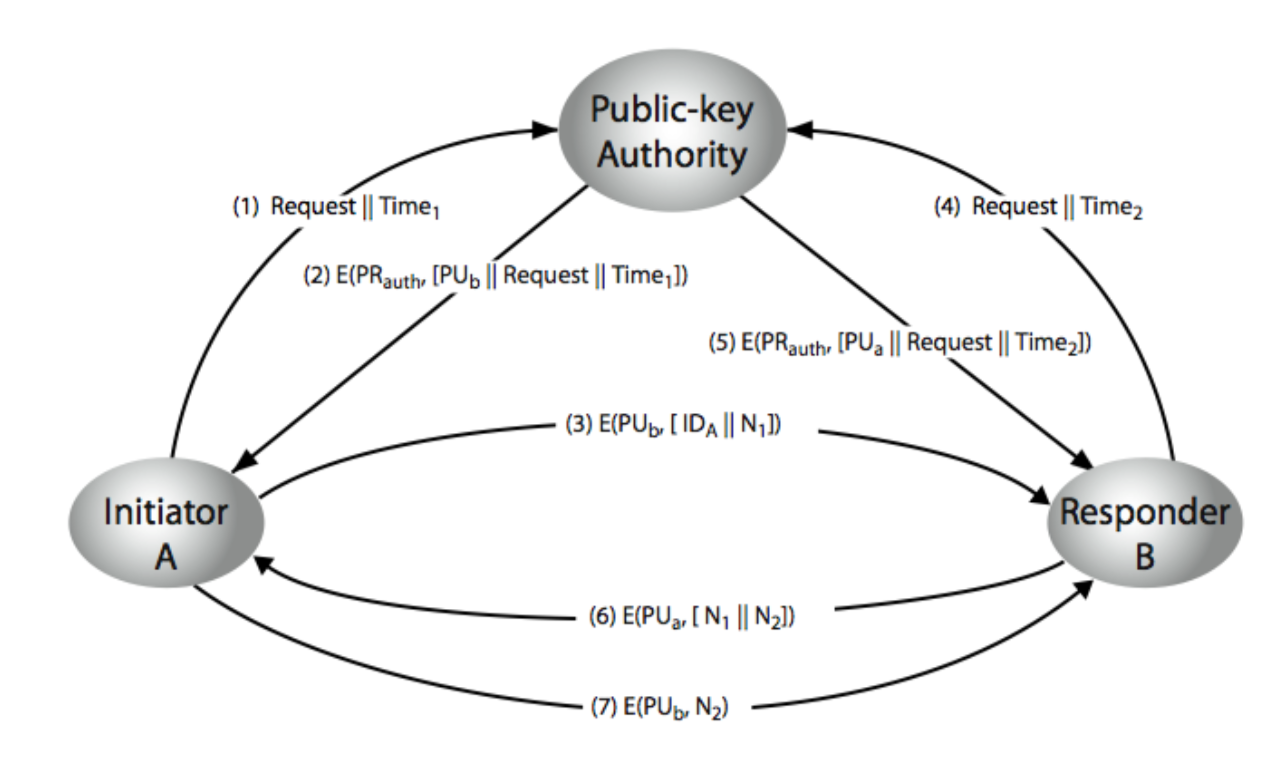
\includegraphics[width= 250pt]{pka.png}
\subsubsection{Public-key certificates}
\begin{itemize}
    \item allow key exchange without real-time access to PKA
    \item certificate binds identity to public key (usually with other info e.g. period of validity)
    \item all contents \textbf{signed} by a trusted PKA or Certificate Authority (i.e. Verisign)
    \item Can be verified by anyone who knows that PKA's public key
\end{itemize}
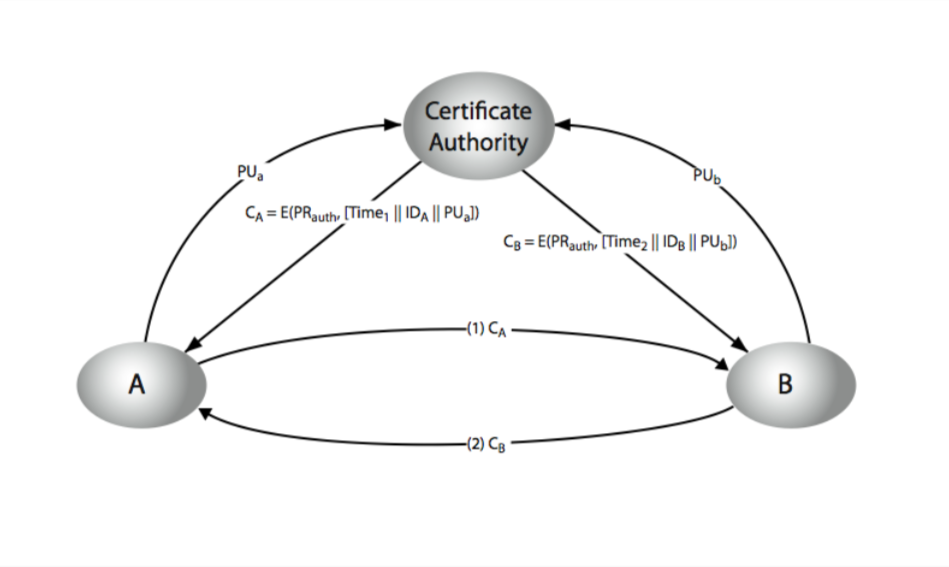
\includegraphics[width= 250pt]{ca.png}
\subsubsection{Public-key distribution of secret keys}
\begin{itemize}
    \item use previous methods to obtain public-key
    \item can use for secrecy or authentication
    \item but, public-key algorithms are slow
    \item usually we want symmetric key encryption to protect message contents, so we need a session key
    \item there are several alternatives for negotiating a suitable session
\end{itemize}
\subsubsection{Diffie-Hellman Key Exchange}
\begin{itemize}
    \item was the first public-key type scheme proposed by Diffie \& Hellman in 1976
    \item practical method for public exchange of a secret key
    \item used in a number of commercial products
    \item public key distribution scheme cannot be used to exchange an arbitrary message, but can be used to establish a common secret key between two participants
    \item key value depends on participants and their priv/pub key information
    \item based on exponentiation in a finite (Galois) field (modulo a prime or polynomial, easy)
    \item security relies on difficulty of computing discrete logarithms (similar to factoring) - hard
\end{itemize}
How do we set up D-H?
\begin{itemize}
    \item both users agree on global parameters: large prime int or polynomial $q$, $a$ being a primitive root modulo $q$
    \item $a$ and $q$ can be transmitted in the clear
    \item each user then generates their key, by choosing a secret key (number): $x_A < q$, and computing their \textbf{public key:} $y_A = a^{x_A} mod q$
    \item each user then publicises their $y_A$
    \item the shared session key for two users A and B is $K_{AB}$
    $$K = a^{x_A + x_B} mod q$$
    $$= y_{A}^{x_B} mod q$$ (which B can compute)
    $$= y_{B}^{x_A} mod q$$ (which A can compute)
    \item $K$ is used as a session key in symmetric encryption scheme between Alice and Bob
    \item attacker needs an $x$ (secret key), must solve discrete logarithm problem 
\end{itemize}
\section{Message Authentication}
\begin{itemize}
    \item sometimes we want to verify integrity/authenticity of message without needing confidentiality
    \item message authentication is the answer
    \item three ways: \textbf{message encryption}, \textbf{message authentication code (MAC)}, \textbf{hash function}
    \item we need authentication in these situations:
    \begin{enumerate}
        \item disclosure
        \item traffic analysis
        \item masquerade
        \item content modification
        \item sequence modification
        \item timing modification
        \item source repudiation
        \item destination repudiation
    \end{enumerate}
\end{itemize}
\subsection{Message Encryption}
Ciphertext of the entire message serves as its authenticator
\subsection{Message Authentication Code (MAC)}
A function of the message and a secret key that produces a fixed length value. This value serves as authenticator
\begin{itemize}
    \item generated by algorithm that creates a small, fixed-sized block
    \item algorithm depends on both message $M$ and some secret key $K$ such that $MAC = C(K,M)$, where $C$ is the MAC function
    \item similiar to encryption, but reversibility is not required (and often not implemented)
    \item appended to message to allow authentication
    \item receiver performs same computation on message and checks that it matches MAC, if so sender and integrity of message is verified
    \item we can also use MAC with encrypted messages using seperate keys for each process
    \item can encrypt message before or after MAC step (encrypting after protects against chosen ciphertext attacks, but more complex to implement)
    \item useful for when we only need authentication, even in longer term
    \item MAC is not digital signature: not unique. Many messages potentially have same MAC, but finding collisions assumed to be difficult
\end{itemize}
Requirements for MAC
\begin{enumerate}
    \item knowing a message and MAC, it is infeasible to find another message with the same MAC
    \item uniformly distributed: for $M$ and $M'$, probability that $C(K,M) = C(K,M')$ is $\frac{1}{2^n}$
    \item MAC should depend on all bits of the message equally
\end{enumerate}
We can also use symmetric ciphers for MACs.
\\e.g., we can use any block cipher chaining mode and then use the final block as the MAC
\\\textbf{Data Authentication Algorithm (DAA)} \textit{was} a popular MAC based on DES-CBC that used an IV of zero and a zero-pad of the final block. It encrypted message using DES-CBC, and sent just the final block (or leftmost $M$ bits \footnote{$16\leq M \leq 64$} of final block). However, this yields a final MAC that is too small to be secure
\section{Hashing Algorithms}
Hash functions transform messages of an arbitrary length to a fixed size $h = H(M)$. Hash functions are public, and typically \textbf{don't} use a key. We can compare hashes to detect changes to message. Most frequent applications of hashing are to create a digital signature for a file (e.g. \textbf{MD5}, \textbf{SHA})
\subsection{Requirements for hash functions}
\begin{itemize}
    \item can be applied to any size message $M$
    \item produces fixed-length output $h$
    \item is easy to compute $h = H(M)$ for any message $M$
    \item has one-way property: given $h$, infeasible to find $M$
    \item has weak collision resistance: given $x$, is infeasible to find $y$ such that $H(x) = H(y)$
    \item has strong collision resistance: infeasible to find an $x,y$ pair such that $H(x) = H(y)$
\end{itemize}
\subsection{Simple Hash Functions}
several proposals for simple functions, based on XOR of message blocks
\\Message is arranged into ~$ \frac{m}{n} $ blocks, where $m$ = message length and $n$ = hash size
\\RXOR (rotate XOR), generally not crypotographically secure
\subsection{Secure Hash Algorithm (SHA)}
\begin{itemize}
    \item originally designed by NIST and NSA in 1993
    \item revised as SHA-1 in 1995
    \item US standard for use with DSA signature scheme (FIPS 180-1 1995, RFC3174)
    \item based on MD4 but with some differences (produces 160-bit hash values)
    \item SHA-1 is no longer considered secure, SHA2 recommended
\end{itemize}
\subsection{In summary}
\begin{itemize}
    \item Hash Functions
    \begin{itemize}
        \item condense arbitrary size message to fixed size by processing message in blocks through some unkeyed compression function
    \end{itemize}
    \item Message Authentication Code (MAC)
    \begin{itemize}
        \item fixed size authenticator for some message using either block cipher mode or keyed hash
    \end{itemize}
\end{itemize}
\section{Introduction to Secure SHell (SSH)}
\subsection{What is SSH?}
\begin{itemize}
    \item SSH provides secure channel over unsecured network in client-server architecture
    \item SSH client connects to SSH server
    \item provides Confidentiality and Integrity, with authentication
    \item SSH-1 and SSH-2 versions
\end{itemize}
\subsection{Overview}
There are two phases to SSH
\begin{itemize}
    \item session key generation
    \item public-key based authentication (optional)
\end{itemize}
SSH uses several crypto primitives:
\begin{itemize}
    \item chacha20-poly1305
    \item aes128-ctr
    \item aes256-ctr
    \item aes128-gcm
    \item aes256-gcm
    \item aes128-cbc
    \item aes192-cbc
    \item aes256-cbc
    \item 3des-cbc
    \item Diffie-Hellman key exchange
    \item HMAC (hashed MAC)
\end{itemize}
\subsection{Session Key Generation}
\begin{enumerate}
    \item TCP handshake
    \item SSH handshake begins
    \item client shares crypto algorithms it can support
    \item server agrees on one of them
    \item client and server begin DH key exchange and generate a session key
    \item each message must contain a MAC to verify packet integrity
    \begin{itemize}
        \item this MAC is calculated from the shared secret, the packet seq#, and the actual message contents
    \end{itemize}
\end{enumerate}
\subsection{User authentication}
\begin{itemize}
    \item password-based (encrypted with session key)
    \item public-key based (recommended!)
    \begin{itemize}
        \item user sends public key to server
        \item it is saved in \~/.ssh/authorised_keys file serverside
        \item now user can log in without password, using their private key to authenticate
    \end{itemize}
\end{itemize}
\section{Introduction to Secure Sockets Layer (SSL)}
\subsection{Problems in web security}
\begin{itemize}
    \item Confidentiality
    \begin{itemize}
        \item eavesdropping on connections
        \item theft of info from server or client
        \item solution: \textbf{encryption}
    \end{itemize}
    \item Integrity
    \begin{itemize}
        \item modification of user data
        \item trojan horse browser
        \item modification of memory
        \item modification of message traffic in transit
        \item solution: \textbf{cryptographic checksums}
    \end{itemize}
    \item Authentication
    \begin{itemize}
        \item Impersonation of users
        \item data forgery
        \item solution: \textbf{cryptographic signatures}
    \end{itemize}
    \item Location of the threat:
    \begin{itemize}
        \item web server
        \item web browser
        \item network traffic
    \end{itemize}
\end{itemize}
\subsection{What is SSL?}
\begin{itemize}
    \item \textbf{transport layer} security service
    \item developed by Netscape originally, v3 with public input
    \item subsequently became internet standard known as TLS (transport layer security)
    \item uses TCP for reliable service
    \item has two layers of protocols
    \begin{enumerate}
        \item L1: SSL Record Protocol
        \item L2: Handshake, change cipher, alert
    \end{enumerate}
    \item Handshake for session init, record for data transfer, alert for message passing, change cipher for changing crypto method
\end{itemize}
%SSL STACK IMAGE HERE
SSL Connection:
\begin{itemize}
    \item transient, p2p communications link associated with 1 SSL \textbf{session}
    \item Dimensions:
    \begin{itemize}
        \item server and client random byte
        \item server write MAC secret: secret key for MAC
        \item client write MAC secret: secret key for MAC
        \item server write key: encryption key
        \item client write key: encryption key
        \item init vectors
        \item sequence numbers for packets
    \end{itemize}
\end{itemize}
SSL Session:
\begin{itemize}
    \item association between client and server
    \item created by handshake protocol
    \item \textbf{defines} a set of cryptographic parameters
    \item may be shared by \textbf{multiple} SSL connections
    \item Dimensions:
    \begin{itemize}
        \item session identifier generated by server
        \item peer certificate (X.509 v3)
        \item compression method
        \item cipher specification
        \item master secret
        \item is resumable?
    \end{itemize}
\end{itemize}
\subsection{SSL Record Protocol Services}
\begin{itemize}
    \item message integrity: using a MAC with a shared secret key, similar to HMAC but with some differences
    %maybe include code snippet here? lecture9slide11
    \item confidentiality: use symmetric encryption with a shared secret key defined by handshake protocol
    \item AES, IDEA, RC2-40, DES-40, DES, 3DES, Fortezza, RC4-40, RC4-128
    \item message is optionally compressed before encryption
\end{itemize}
%include image from lec9slide13
\subsection{SSL Change Cipher Spec Protocol}
\begin{itemize}
    \item one of 3 SSL specific protocols which use the SSL record protocol
    \item single message consists of just one byte: 1
    \item causes pending state to become current, updating cipher suite in use
    \item sent after just-negotiated cipherspec and keys
\end{itemize}
\subsection{SSL Alert Protocol}
\begin{itemize}
    \item conveys SSL-related alerts to peer entity
    \item 2 byte messages
    \item severity indicated in the first byte (warning or fatal)
    \item specific alert in the second byte
    \begin{itemize}
        \item fatal: unexpected message, bad record mac, decompression failure, handshake failure, illegal parameter
        \item warning: close notify, no cert, bad cert, unsupported cert, cert revoked, cert expired, cert unknown
    \end{itemize}
    \item compressed and encrypted like all SSL data
\end{itemize}
\end{document}
